% Created by tikzDevice version 0.12.3.1 on 2021-06-03 11:50:02
% !TEX encoding = UTF-8 Unicode
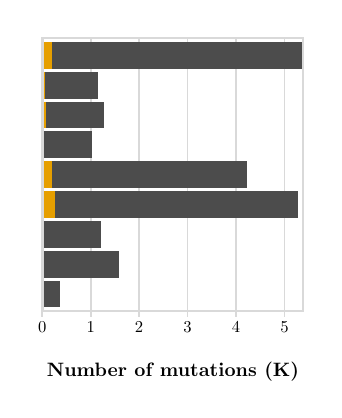
\begin{tikzpicture}[x=1pt,y=1pt]
\definecolor{fillColor}{RGB}{255,255,255}
\path[use as bounding box,fill=fillColor,fill opacity=0.00] (0,0) rectangle (103.28,130.99);
\begin{scope}
\path[clip] (  5.25, 28.30) rectangle ( 99.78,127.49);
\definecolor{drawColor}{gray}{0.85}

\path[draw=drawColor,line width= 0.6pt,line join=round] (  5.25, 28.30) --
	(  5.25,127.49);

\path[draw=drawColor,line width= 0.6pt,line join=round] ( 22.77, 28.30) --
	( 22.77,127.49);

\path[draw=drawColor,line width= 0.6pt,line join=round] ( 40.28, 28.30) --
	( 40.28,127.49);

\path[draw=drawColor,line width= 0.6pt,line join=round] ( 57.80, 28.30) --
	( 57.80,127.49);

\path[draw=drawColor,line width= 0.6pt,line join=round] ( 75.31, 28.30) --
	( 75.31,127.49);

\path[draw=drawColor,line width= 0.6pt,line join=round] ( 92.83, 28.30) --
	( 92.83,127.49);
\definecolor{fillColor}{gray}{0.30}

\path[fill=fillColor] (  8.74,116.17) rectangle ( 99.78,125.87);
\definecolor{fillColor}{RGB}{230,159,0}

\path[fill=fillColor] (  5.25,116.17) rectangle (  8.74,125.87);
\definecolor{fillColor}{gray}{0.30}

\path[fill=fillColor] (  6.25,105.39) rectangle ( 25.25,115.09);
\definecolor{fillColor}{RGB}{230,159,0}

\path[fill=fillColor] (  5.25,105.39) rectangle (  6.25,115.09);
\definecolor{fillColor}{gray}{0.30}

\path[fill=fillColor] (  6.56, 94.61) rectangle ( 27.44,104.31);
\definecolor{fillColor}{RGB}{230,159,0}

\path[fill=fillColor] (  5.25, 94.61) rectangle (  6.56,104.31);
\definecolor{fillColor}{gray}{0.30}

\path[fill=fillColor] (  5.25, 83.83) rectangle ( 23.22, 93.53);

\path[fill=fillColor] (  8.93, 73.05) rectangle ( 79.36, 82.75);
\definecolor{fillColor}{RGB}{230,159,0}

\path[fill=fillColor] (  5.25, 73.05) rectangle (  8.93, 82.75);
\definecolor{fillColor}{gray}{0.30}

\path[fill=fillColor] (  9.87, 62.27) rectangle ( 97.73, 71.97);
\definecolor{fillColor}{RGB}{230,159,0}

\path[fill=fillColor] (  5.25, 62.27) rectangle (  9.87, 71.97);
\definecolor{fillColor}{gray}{0.30}

\path[fill=fillColor] (  5.81, 51.48) rectangle ( 26.62, 61.19);
\definecolor{fillColor}{RGB}{230,159,0}

\path[fill=fillColor] (  5.25, 51.48) rectangle (  5.81, 61.19);
\definecolor{fillColor}{gray}{0.30}

\path[fill=fillColor] (  5.25, 40.70) rectangle ( 32.87, 50.41);

\path[fill=fillColor] (  5.43, 29.92) rectangle ( 11.78, 39.62);
\definecolor{fillColor}{RGB}{230,159,0}

\path[fill=fillColor] (  5.25, 29.92) rectangle (  5.43, 39.62);

\path[draw=drawColor,line width= 1.1pt,line join=round,line cap=round] (  5.25, 28.30) rectangle ( 99.78,127.49);
\end{scope}
\begin{scope}
\path[clip] (  0.00,  0.00) rectangle (103.28,130.99);
\definecolor{drawColor}{gray}{0.85}

\path[draw=drawColor,line width= 0.6pt,line join=round,line cap=rect] (  5.25, 28.30) --
	(  5.25,127.49);
\end{scope}
\begin{scope}
\path[clip] (  0.00,  0.00) rectangle (103.28,130.99);
\definecolor{drawColor}{gray}{0.85}

\path[draw=drawColor,line width= 0.6pt,line join=round] (  5.25, 26.55) --
	(  5.25, 28.30);

\path[draw=drawColor,line width= 0.6pt,line join=round] ( 22.77, 26.55) --
	( 22.77, 28.30);

\path[draw=drawColor,line width= 0.6pt,line join=round] ( 40.28, 26.55) --
	( 40.28, 28.30);

\path[draw=drawColor,line width= 0.6pt,line join=round] ( 57.80, 26.55) --
	( 57.80, 28.30);

\path[draw=drawColor,line width= 0.6pt,line join=round] ( 75.31, 26.55) --
	( 75.31, 28.30);

\path[draw=drawColor,line width= 0.6pt,line join=round] ( 92.83, 26.55) --
	( 92.83, 28.30);
\end{scope}
\begin{scope}
\path[clip] (  0.00,  0.00) rectangle (103.28,130.99);
\definecolor{drawColor}{RGB}{0,0,0}

\node[text=drawColor,anchor=base,inner sep=0pt, outer sep=0pt, scale=  0.60] at (  5.25, 20.92) {0};

\node[text=drawColor,anchor=base,inner sep=0pt, outer sep=0pt, scale=  0.60] at ( 22.77, 20.92) {1};

\node[text=drawColor,anchor=base,inner sep=0pt, outer sep=0pt, scale=  0.60] at ( 40.28, 20.92) {2};

\node[text=drawColor,anchor=base,inner sep=0pt, outer sep=0pt, scale=  0.60] at ( 57.80, 20.92) {3};

\node[text=drawColor,anchor=base,inner sep=0pt, outer sep=0pt, scale=  0.60] at ( 75.31, 20.92) {4};

\node[text=drawColor,anchor=base,inner sep=0pt, outer sep=0pt, scale=  0.60] at ( 92.83, 20.92) {5};
\end{scope}
\begin{scope}
\path[clip] (  0.00,  0.00) rectangle (103.28,130.99);
\definecolor{drawColor}{RGB}{0,0,0}

\node[text=drawColor,anchor=base,inner sep=0pt, outer sep=0pt, scale=  0.70] at ( 52.51,  4.86) {\bfseries Number of mutations (K)};
\end{scope}
\end{tikzpicture}%
